\chapter{Pruebas}
En este capítulo se expondrán los experimentos ejecutados en los nodos de computación del CESGA y los resultados obtenidos. El experimento se divide en dos secciones: el análisis principal, el de tiempos de ejecución, y un análisis complementario de escalabilidad de paralelización. Los experimentos de tiempos de ejecución se dividen a su vez en búsquedas de subconjuntos con centros aleatorios y en búsquedas sobre nubes completas.

\section{Plan de Verificación y Corrección Global}
Como paso previo al análisis de rendimiento, se diseñó un script de pruebas unitarias automatizadas para verificar la fidelidad de los nuevos algoritmos orientados a la poda en nodos hoja. Para cada una de las configuraciones evaluadas en este capítulo, se contrastaron los resultados de vecindad devueltos por las variantes optimizadas frente a los resultados reportados por la implementación base del Octree lineal clásico. La verificación produjo una coincidencia del 100\%, por tanto se pasó al estudio de los resultados temporales, con la garantía de que en las podas se descartan únicamente regiones del espacio geométrico disjuntas al kernel.

Adicionalmente, se usó el modo de debug implementado para tener una medida de la efectividad teórica de las podas, más allá de saber si son eficientes temporalmente o no. En la Figura \ref{fig:metricas_poda_lille} se recoge el porcentaje puntos analizados después de calcular la poda y el porcentaje de puntos que resultaron ser vecinos en relación al número de puntos totales de cada hoja para la nube de puntos de \textit{Lille\_0}. Los resultados a lo largo de las diferentes nubes fueron muy consistentes, siendo este dataset lo suficientemente representativo. Para obtener estos resultados se usó una muestra de 80 búsquedas con centros aleatorios. El caso ideal es que el número de puntos analizados después de la poda y el número de puntos vecinos sea el mismo. El tamaño de los kernels se muestra representado como la media de la relación entre el radio y el tamaño de las hojas que se podan, de forma que se pueda tener una visión más independiente al dataset de cómo funciona la poda con diferentes tamaños de búsqueda. 

Los porcentajes mostrados indican un comportamiento claro: el modo polar poda de manera aceptable en las búsquedas con kernel esférico, pero apenas poda en búsquedas cúbicas. Por el contrario, el modo cartesiano realiza podas que están cerca de ser ideales para geometría cúbica, en cambio descarta muy pocos puntos en búsquedas esféricas. En la poda polar hay otra tendencia clara observable, y es que a medida que el radio es más pequeño en relación a la magnitud de los octantes, se descarta un mayor porcentaje de puntos y se reduce la diferencia con el porcentaje de vecinos. Por otra parte, en el reordenamiento cartesiano sobre kernel esférico ocurre lo contrario, se abre esa distancia a medida que aumenta el radio de búsqueda. Aún así, esta degradación es muy leve y continúan siendo podas muy efectivas (no se supera el 25\% de diferencia entre puntos recorridos y aceptados en ningún caso).

\begin{figure}[htbp]
    \centering
    \begin{subfigure}{0.99\textwidth}
        \centering
        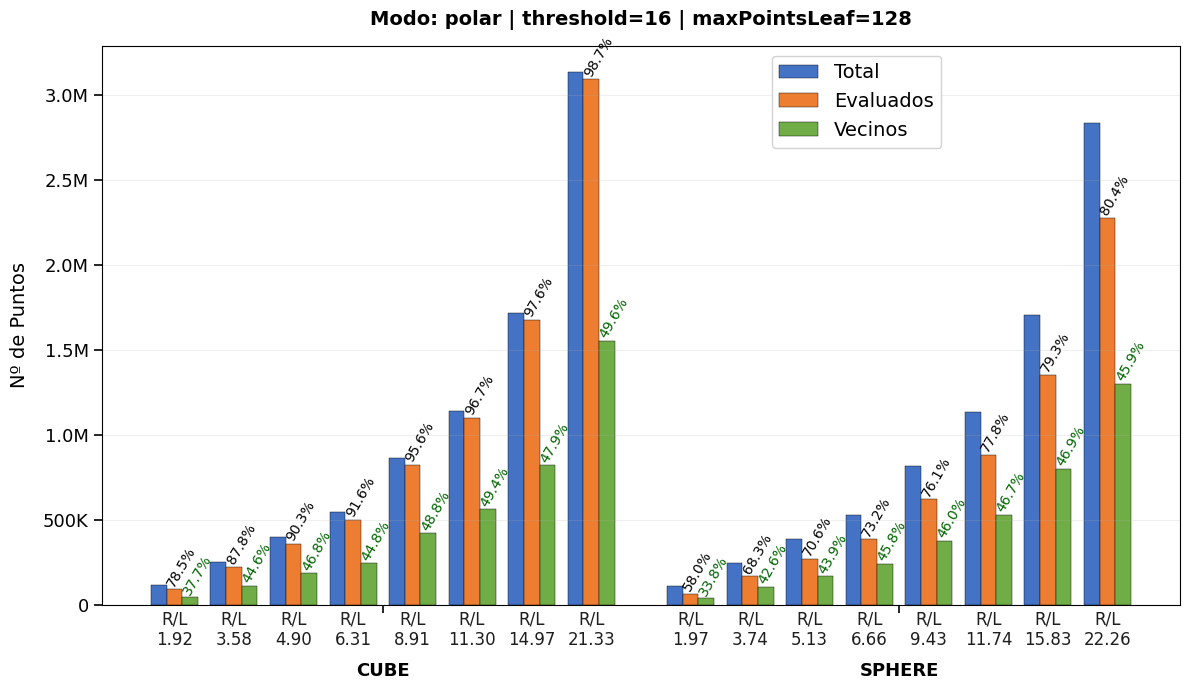
\includegraphics[width=1\textwidth]{figuras/metodologia/metricas_poda_lille_polar.png}
        \caption{Modo de reordenamiento polar}
        \label{fig:metricas_poda_lille_polar}
    \end{subfigure}
    
    \vspace{0.5cm}
    
    \begin{subfigure}{0.99\textwidth}
        \centering
        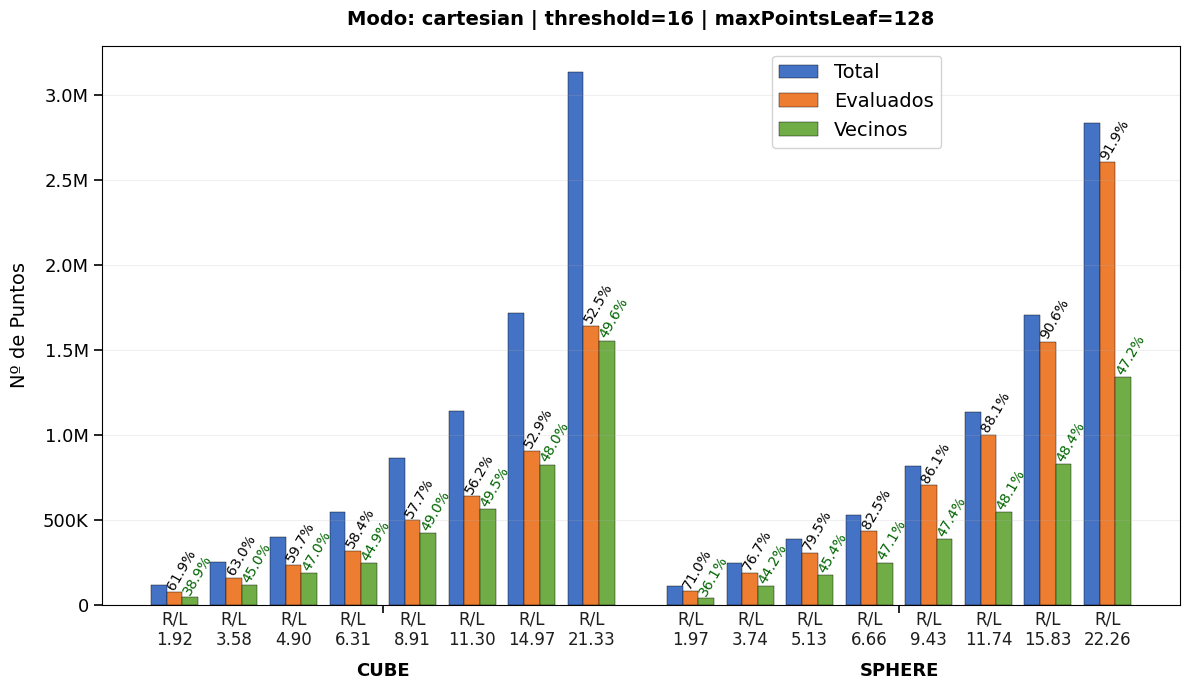
\includegraphics[width=1\textwidth]{figuras/metodologia/metricas_poda_lille_cartesian.png} 
        \caption{Modo de reordenamiento cartesiano}
        \label{fig:metricas_poda_lille_cart}
    \end{subfigure}
    \caption{Efectividad teórica de cada modo de poda sobre el dataset \textit{Lille\_0}, sobre kernels cúbicos y esféricos de diferentes tamaños, usando un tamaño máximo de hoja de 128 puntos.}
    \label{fig:metricas_poda_lille} 
\end{figure}


\section{Rendimiento de búsquedas de vecinos paralelas con centros aleatorios}
Estos experimentos exploran la eficiencia temporal en la ejecución de un lote de 10.000 consultas espaciales con centros distribuidos aleatoriamente. Cada configuración se repitió 5 veces, tomando como métrica el tiempo medio de ejecución. Cabe destacar que se empleó una paralelización a escala de 40 núcleos en todas las ejecuciones. Se usaron todas las nubes de puntos descritas en el apartado 3.4, variando los siguientes hiperparámetros:
\begin{itemize}
    \item \textbf{Modo de reordenamiento}. Se probaron tanto los dos modos de poda propios como la versión de búsqueda sobre un Octree lineal base propuesta por Viñambres et al \cite{Vinambres}.
    \item \textbf{Algoritmo de búsqueda}. Se sometieron a pruebas los dos métodos estudiados y modificados: \textit{neighborsPrune} y \textit{neighborsStruct} .
    \item  \textbf{Kernel}. Los dos kernels tridimensionales soportados: cubo y esfera.
    \item  \textbf{Algoritmos de SFC}. Se usaron tanto los códigos de Morton como los de Hilbert. Sin embargo, no se analizaron los resultados por separado, eso está fuera del alcance del trabajo. Se incluyeron para promediar los resultados con los dos \textit{encoders} y tener una visión más contrastada de los resultados.
    \item  \textbf{Radio}. Se dividieron las nubes en tres grupos: de densidad alta, media y baja, según la naturaleza de la nube. Para cada grupo se ejecutó una selección de 8 radios distintos adaptada a la cantidad de vecinos aproximada que producirán.
    \item \textbf{Tamaño de hoja (número máximo de puntos)}. Este parámetro es de los más críticos para este trabajo. Puede influir directamente en el rendimiento temporal de la poda. Se probaron valores de $128, 256, 512, 768, 1024$
    \item \textbf{Umbral de poda (threshold)}. Parámetro dedicado de esta optimización. Puede presentar cambios en el rendimiento, midiendo en qué punto deja de ser rentable o no el algoritmo de poda. Se probaron los valores $16, 64, 100$.
\end{itemize}

A continuación, se muestran los resultados obtenidos. Para empezar, se visualiza el tiempo de ejecución medio, dado un radio y una geometría de búsqueda, de cada combinación de algoritmo y reordenación local para los diferentes tamaños de hoja propuestos. En las Figuras \ref{fig:subset_barras_dales} y \ref{fig:subset_barras_bild} se ven los resultados variando el radio y la nube de puntos usada.

\begin{figure}[htbp]
    \centering
    \begin{subfigure}{0.95\textwidth}
        \centering
        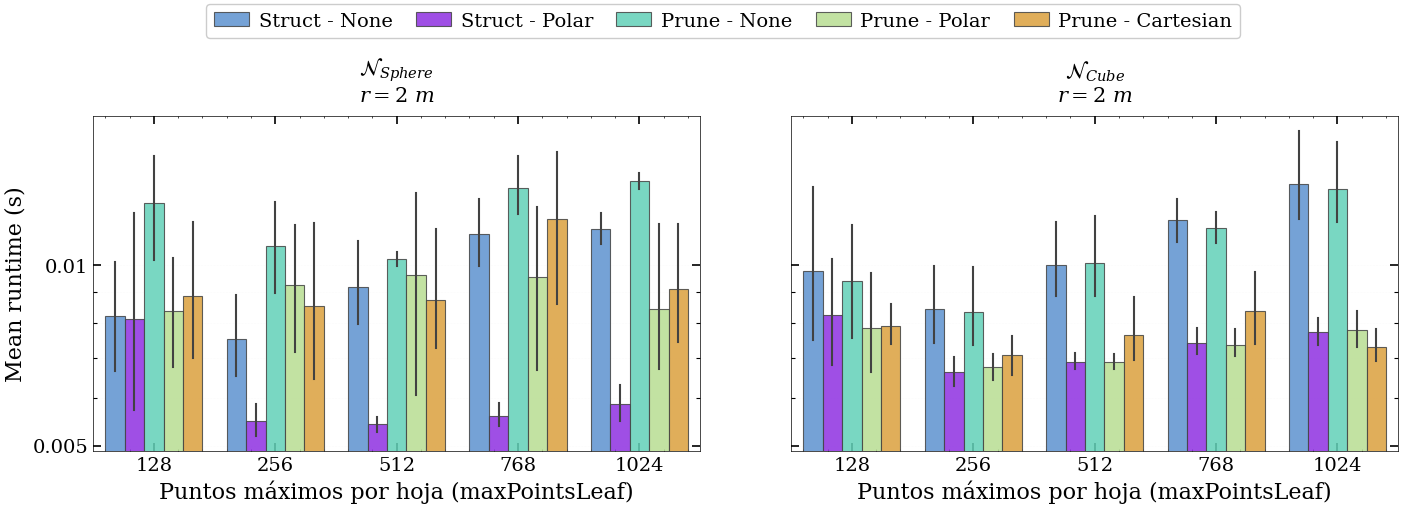
\includegraphics[width=0.98\textwidth]{figuras/subset/dales_r2.png}
        \label{fig:dales_r2}
    \end{subfigure}
    
    \vspace{0.5cm}
    
    \begin{subfigure}{0.95\textwidth}
        \centering
        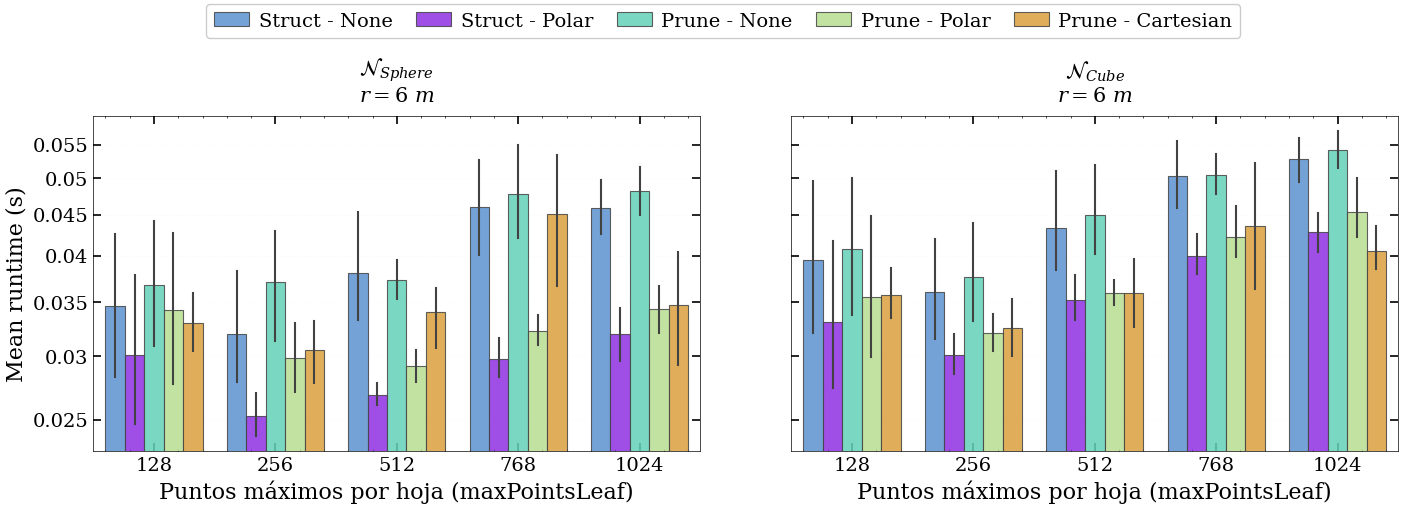
\includegraphics[width=0.98\textwidth]{figuras/subset/dales_r6.png} 
        \label{fig:dales_r6}
    \end{subfigure}
    \caption{Tiempos medios de búsqueda de vecindades de 10.000 puntos aleatorios tomando diferentes radios en \textit{5085\_54320}}
    \label{fig:subset_barras_dales} 
\end{figure}


\begin{figure}[htbp]
    \vspace{0.5cm}
    \centering
    \begin{subfigure}{0.95\textwidth}
        \centering
        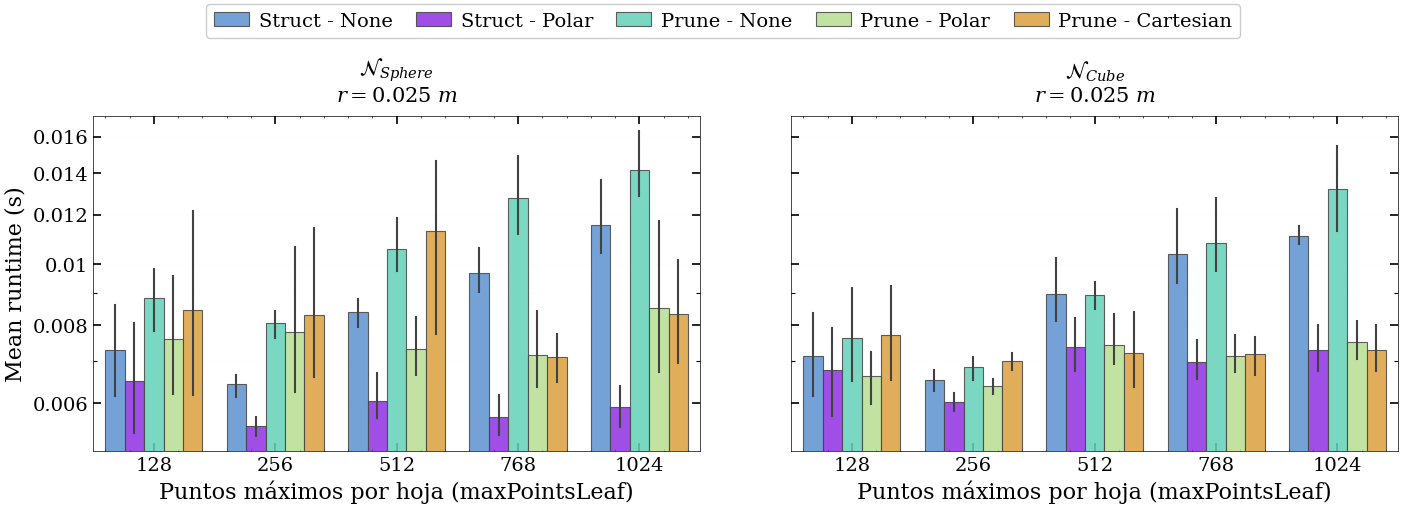
\includegraphics[width=0.98\textwidth]{figuras/subset/bild_r0025.png} 
        \label{fig:bild_r0025}    
        \vspace{0.5cm}

    \end{subfigure} 
    \begin{subfigure}{0.95\textwidth}
        \centering
        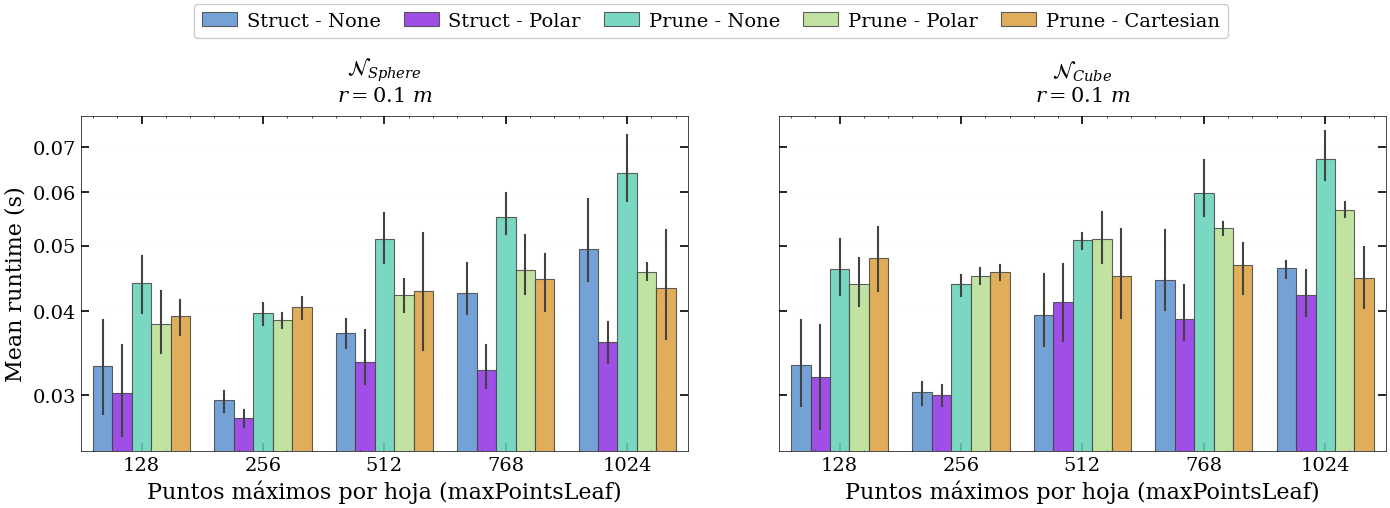
\includegraphics[width=0.98\textwidth]{figuras/subset/bild_r01.png} 
        \label{fig:bild_r01}
    \end{subfigure}
    \caption{Tiempos medios de búsqueda de vecindades de 10.000 puntos aleatorios tomando diferentes radios en \textit{bildstein\_station1}}
    \label{fig:subset_barras_bild}
\end{figure}


Tal y como se evidencia en las Figuras \ref{fig:subset_barras_dales} y \ref{fig:subset_barras_bild} , los mínimos absolutos de tiempo se alcanzan de manera consistente al configurar un tamaño de nodo hoja fijado en \texttt{256}. Asimismo, destaca la superioridad del algoritmo \textit{neighborsStruct}. Aislando sus dos versiones, las implementaciones que incorporan reordenaciones locales y selectores de rango reportan una aceleración notable del tiempo de ejecución respecto al algoritmo original del Octree lineal, en especial en kernels esféricos. 

En cuanto a los resultados aislados de \textit{neighborsPrune}, en general están alejados, pero tanto el reordenamiento polar como el cartesiano tienen un desempeño similar, en ciertos casos mejor, al algoritmo base. Comparándolos entre ellos, ninguno de los dos reordenamientos aplicados a \textit{neighborsPrune} destaca claramente sobre el otro.

Una tendencia que sí se puede apreciar es que los reordenamientos mantienen el rendimiento de forma más estable a medida que se disparan los tamaños de las hojas, contrastando con la degradación en los tiempos que sufren las implementaciones originales.

Seguidamente, se analiza el impacto combinado de las dos variables de control críticas en el rendimiento de la poda: el tamaño máximo de nodo hoja (\texttt{maxLeaf}) frente al umbral de activación del selector (\texttt{threshold}). Para aislar el efecto del resto de parámetros, ambas variables se contraponen en una matriz bidimensional. 

El valor indexado en cada celda de la matriz corresponde a la media aritmética del \textit{speedup} ($S$) obtenido para el conjunto de radios evaluados. Para evitar que los radios con mayores tiempos absolutos sesguen el mapa de calor, el \textit{speedup} de cada radio $r$ se normaliza dividiendo el tiempo de la configuración actual entre el tiempo mínimo absoluto registrado para ese mismo radio entre todo el espectro de hiperparámetros testados. Finalmente, este indicador se promedia combinando los resultados de ambos kernels de búsqueda (cubo y esfera), respondiendo a la siguiente expresión:

\begin{equation}
    S_{\text{medio}} = \frac{1}{|K| \cdot |R|} \sum_{k \in K} \sum_{r \in R} \frac{T_{\text{optimo}}(k)}{T(k, r, maxLeaf, threshold, algoritmo)}
\end{equation}

\begin{figure}[htbp]
    \centering
    % Primera gráfica (Izquierda)
    \begin{subfigure}[b]{0.48\textwidth}
        \centering
        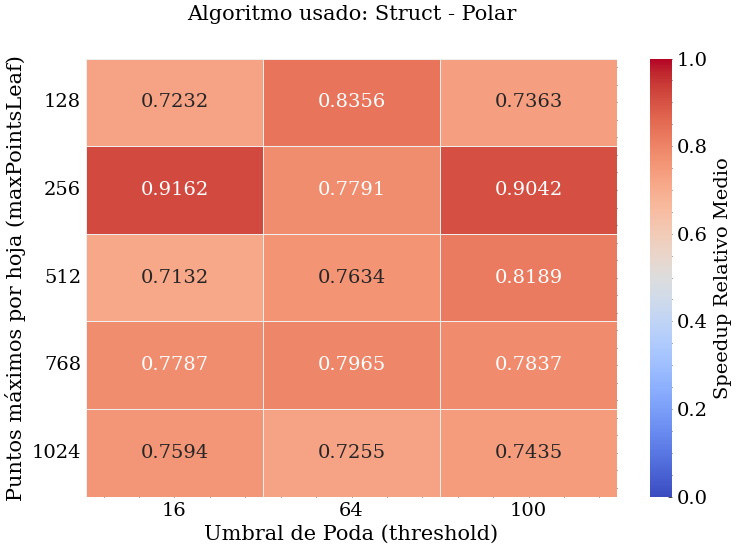
\includegraphics[width=\textwidth]{figuras/subset/heatmap_18train.png}
        \label{fig:heatmapTrain}
    \end{subfigure}
    \hfill 
    \begin{subfigure}[b]{0.48\textwidth}
        \centering
        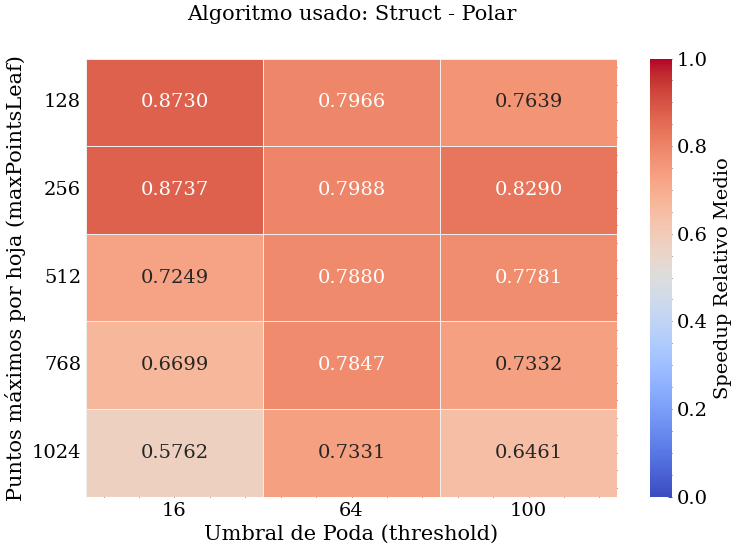
\includegraphics[width=\textwidth]{figuras/subset/heatmap_18test.png}
        \label{fig:heatmapTest}
    \end{subfigure}
    \caption{Análisis del rendimiento temporal de hiperparámetros en las nubes de puntos \textit{Mar18Train} y \textit{Mar18Test}}
    \label{fig:heatmapsHiperparámetros}
\end{figure}

Debido a que la reordenación polar en conjunto con las búsquedas mediante \textit{neighborsStruct} fue la más eficiente, será esa configuración en la que se centrará el estudio de hiperparámetros. Como se puede apreciar en la Figura \ref{fig:heatmapsHiperparámetros},  la combinación más eficiente para el comportamiento del Octree en las nubes del dataset \textit{Hessigheim 3D} se produce con hojas de \texttt{256} puntos y con un umbral de activación de poda (\texttt{threshold}) fijado en \texttt{16} puntos. 

No obstante, distintas distribuciones de puntos en cada dataset provocan que las combinaciones óptimas presenten ligeras variaciones según la nube de puntos analizada. Por este motivo, se evaluó de forma independiente qué par de hiperparámetros favorecía el rendimiento de cada entorno específico. 

Estas configuraciones óptimas personalizadas constituyen las bases de datos con las que se alimentaron los resultados a continuación expuestos. En dichos gráficos se cuantifica el tiempo medio de ejecución de las 10.000 consultas espaciales a medida que se incrementa el radio de búsqueda de forma continua, distribuyendo cada serie como una combinación única de algoritmo de asignación y modo de reordenamiento local. Se pueden ver los resultados para diferentes nubes de puntos en las Figuras \ref{fig:subset_lines_train} y \ref{fig:subset_lines_test}.

Estos valores temporales muestran una continuación de los resultados propuestos en las Figuras \ref{fig:subset_barras_dales} y \ref{fig:subset_barras_bild}, pero pudiéndose apreciar tendencias con la introducción de la variación de radio y presentándose, además, comportamientos disjuntos entre nubes. En el dataset \textit{Mar18\_Train} los tiempos siguen una distribución notablemente uniforme. 
Por otro lado, los valores asociados al algoritmo \textit{neighborsStruct} con poda local son los que dominan en cuanto a eficiencia temporal. Aún así, las podas con el algoritmo de \textit{pruning} básico (destacando el modo cartesiano) presentan un rendimiento equiparable en radios intermedios. Eso sí, en ambos datasets estas ejecuciones se degradan en gran medida al escalar los tamaños de las figuras geométricas de búsqueda.

\begin{figure}[H]
    \centering
    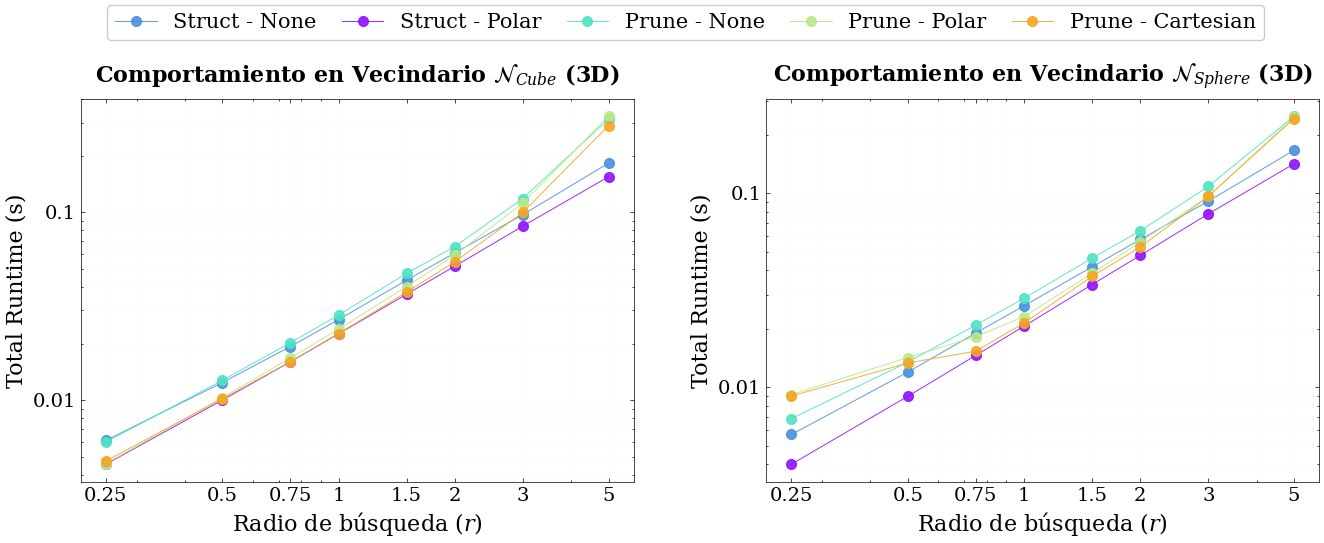
\includegraphics[width=0.95\textwidth]{figuras/subset/lines_18train.png} 
    \caption{Tiempos medios de búsqueda de vecindades de 10.000 puntos aleatorios para diferentes radios en la nube \textit{Mar18\_Train}}
    \label{fig:subset_lines_train}
\end{figure}

\begin{figure}[H]
    \centering
    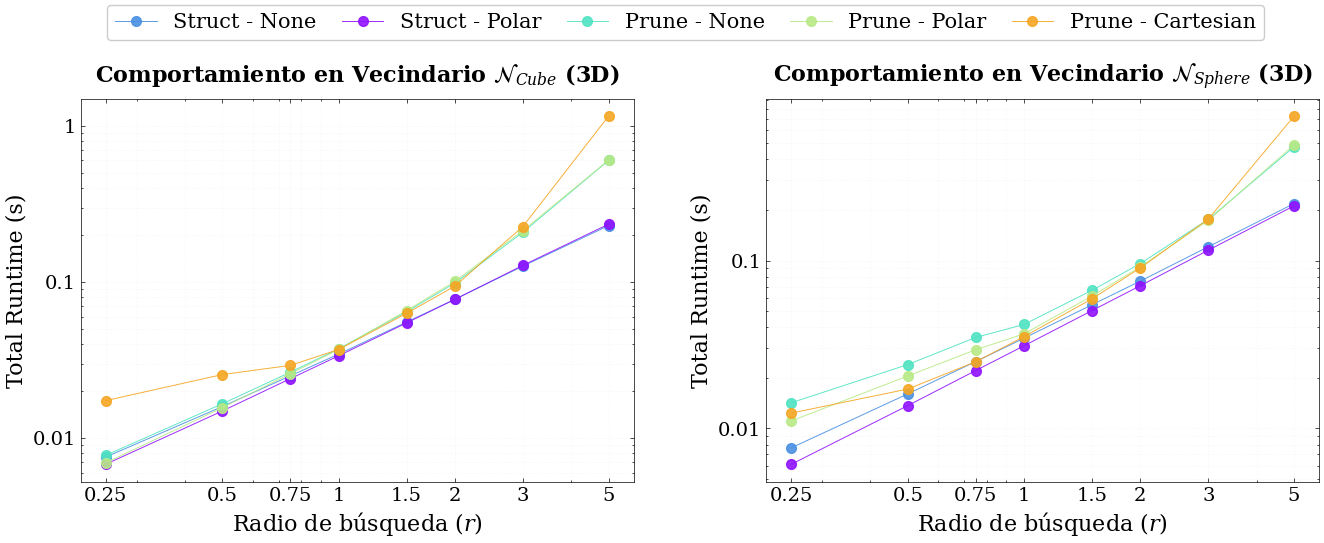
\includegraphics[width=0.95\textwidth]{figuras/subset/lines_18test.png}  
    \caption{Tiempos medios de búsqueda de vecindades de 10.000 puntos aleatorios para diferentes radios en la nube \textit{Mar18\_Test}}
    \label{fig:subset_lines_test}
\end{figure}

\section{Rendimiento de búsquedas de vecinos paralelas sobre toda la nube}
A continuación, se trata un caso de uso muy común en el manejo de nubes de puntos 3D. Estos experimentos evalúan el comportamiento del sistema ante búsquedas masivas secuenciales sobre la totalidad de la nube. Debido a la naturaleza del recorrido y el reparto de carga contiguo por hilos, es necesario explorar las dinámicas de estas consultas de forma independiente. Ya que estas ejecuciones son muy costosas, se seleccionaron un subconjunto de las nubes preparadas, manteniendo variedad entre LiDAR terrestre y aéreo provenientes de diversos datasets. También se mantuvieron fijos los hiperparámetros de \texttt{maxLeaf} y \texttt{threshold}. Se escogió para cada conjunto de nubes un par de valores para estas variables de control que fuese exitoso en los experimentos de centros aleatorios:
\begin{itemize}
    \item \textbf{Perfil de alta densidad}: Nube \textit{bildstein\_station1}. Configuración: \texttt{[256, 64]}
    \item \textbf{Perfil de densidad media}: Nubes  \textit{Mar18\_train} y \textit{Paris\_Luxembourg\_6}. Configuración: \texttt{[128, 64]}
    \item  \textbf{Perfil de baja densidad}: Nubes \textit{PNOA\_2024\_PNR\_489-4672\_NPC01} y \textit{5085\_54320}. Configuración: \texttt{[256, 64]}
\end{itemize}

Adicionalmente, se fijó el algoritmo SFC a los códigos de Hilbert y se fijó una única repetición de las búsquedas.

En la Figura \ref{fig:full_searches} se exploran todos los resultados conseguidos.
\begin{figure}[htbp]
    \centering
    \vspace{0.3cm}
    \begin{subfigure}{0.99\textwidth}
        \centering
        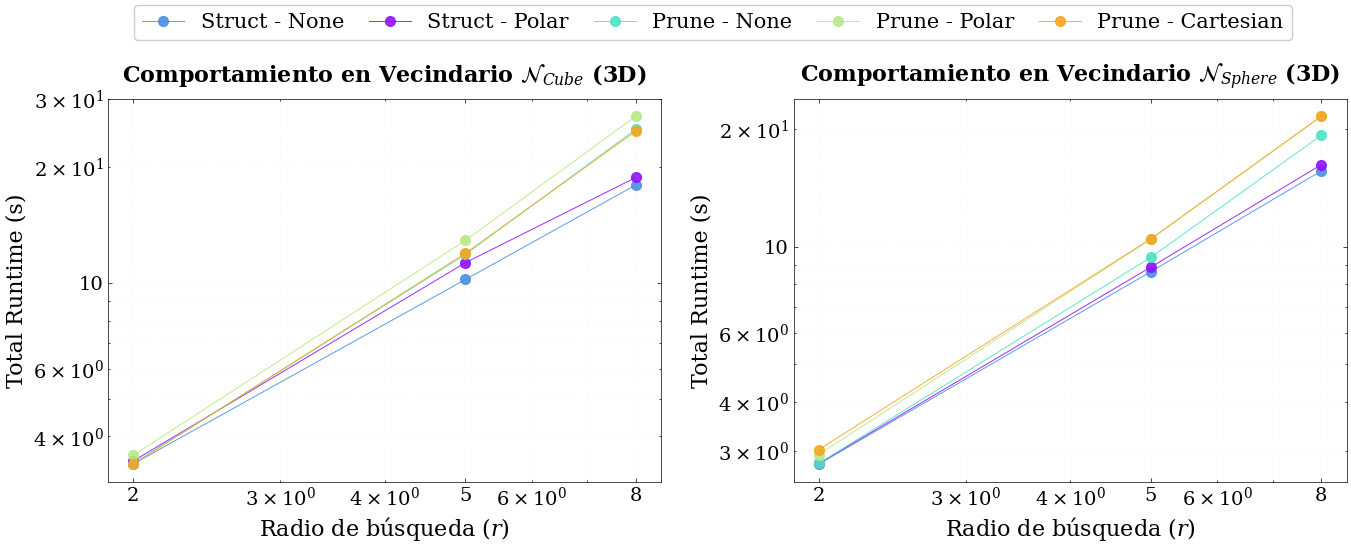
\includegraphics[width=\textwidth]{figuras/full/5085.png}
        \caption{Dataset \textit{5085\_54320}}
        \label{fig:full_a}
    \end{subfigure}
    
    \vspace{0.7cm}
    
    \begin{subfigure}{0.99\textwidth}
        \centering
        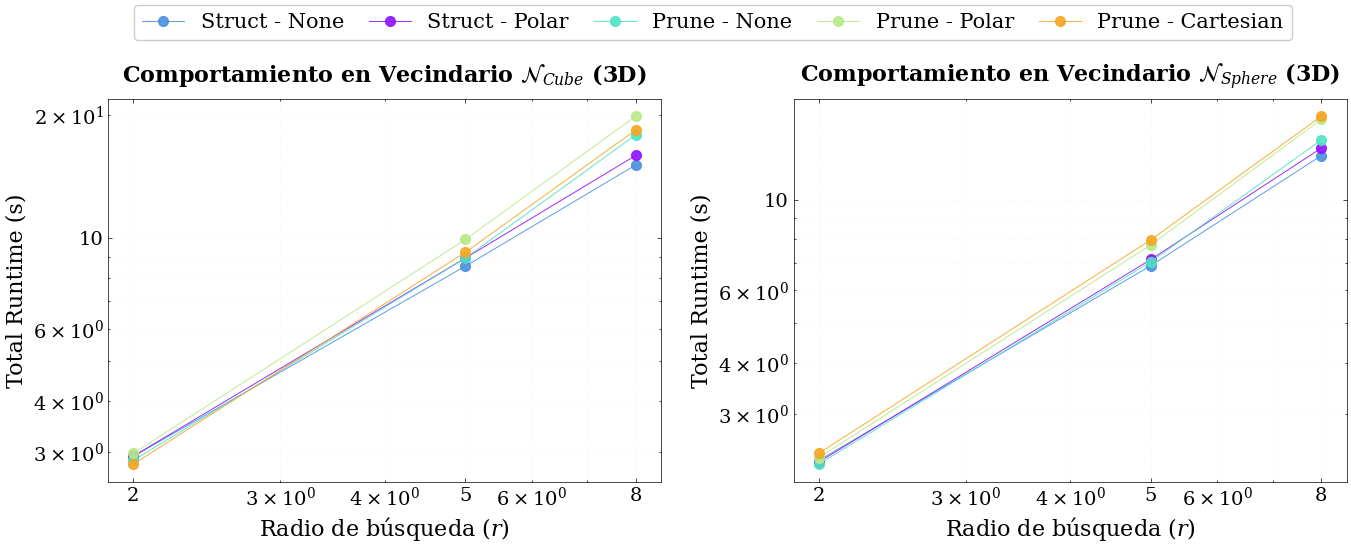
\includegraphics[width=\textwidth]{figuras/full/pnoa.png}
        \caption{Dataset \textit{PNOA\_2024\_PNR\_489-4672\_NPC01}}
        \label{fig:full_b}
    \end{subfigure}
    \vspace{0.7cm}
    \begin{subfigure}{0.98\textwidth}
        \centering
        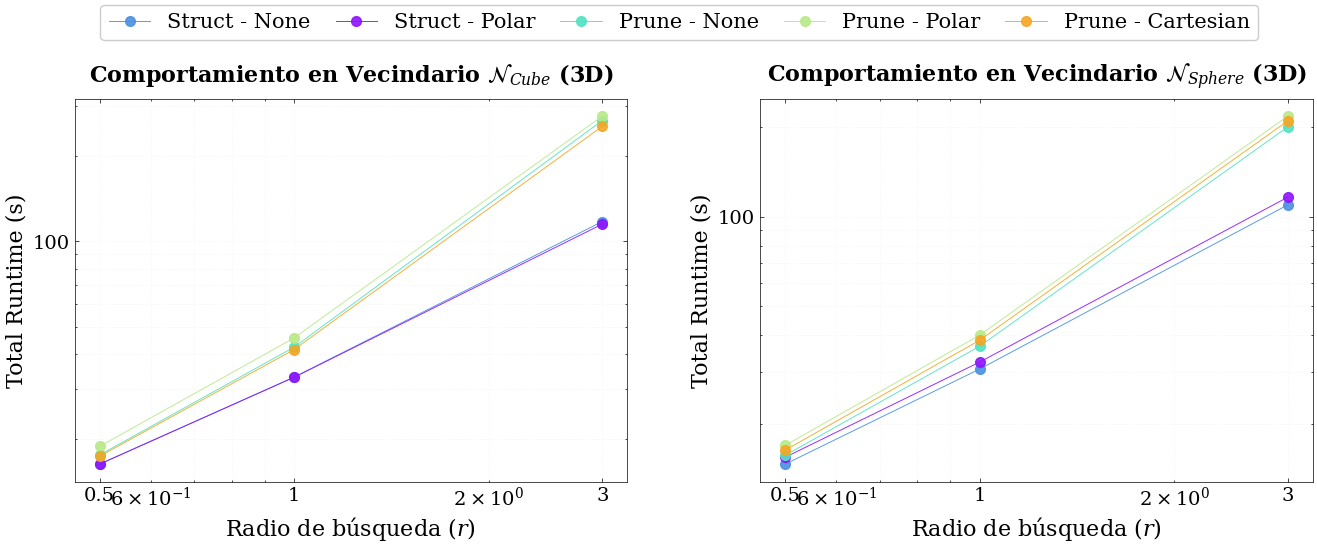
\includegraphics[width=\textwidth]{figuras/full/mar18train.png}
        \caption{Dataset \textit{Mar18\_train}}
        \label{fig:full_c}
    \end{subfigure}
    
    \vspace{0.7cm}
    
\end{figure}

% SEGUNDA PARTE
\begin{figure}[htbp]
    \centering
    \ContinuedFloat 
    \begin{subfigure}{0.98\textwidth}
        \centering
        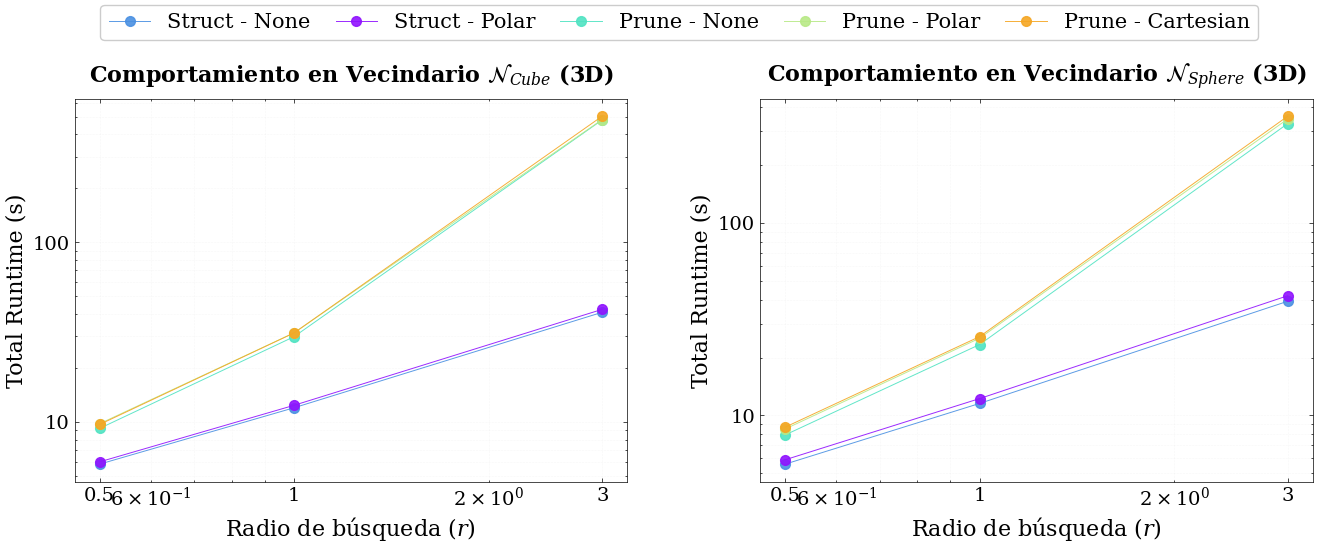
\includegraphics[width=\textwidth]{figuras/full/paris.png}
        \caption{Dataset \textit{Paris\_Luxembourg\_6}}
        \label{fig:full_d}
    \end{subfigure}
    \vspace{0.7cm}

    \begin{subfigure}{0.98\textwidth}
        \centering
        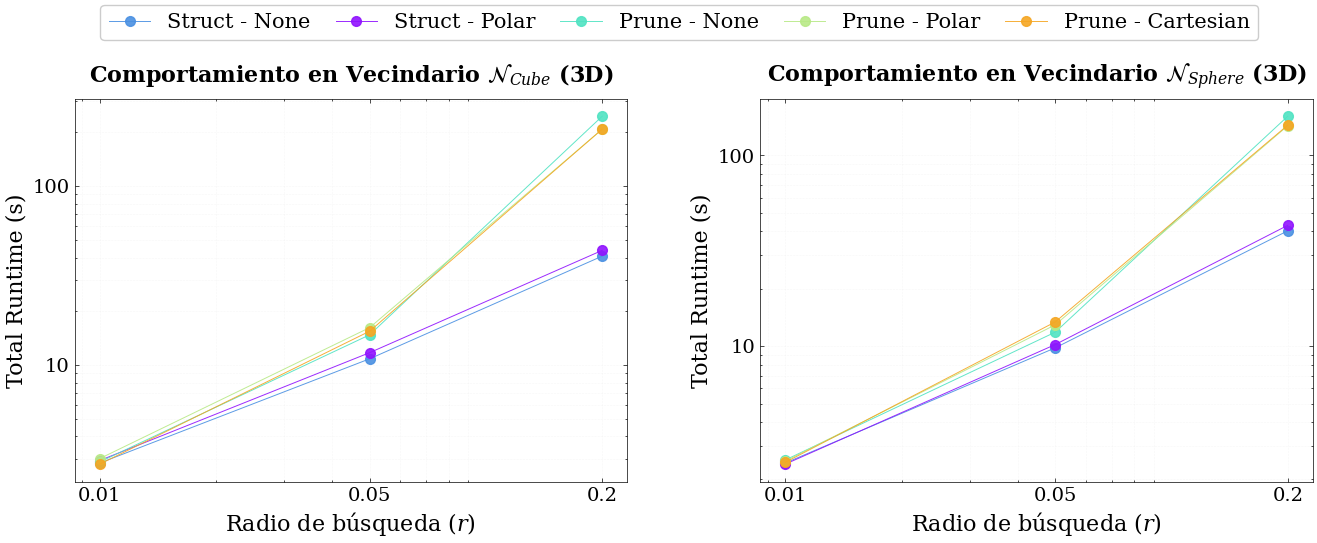
\includegraphics[width=\textwidth]{figuras/full/bild.png}
        \caption{Dataset \textit{bildstein\_station1}}
        \label{fig:full_e}
    \end{subfigure}
    
    \caption{Tiempos de ejecución de búsquedas completas variando el radio operativo sobre kernels esféricos y cúbicos.}
    \label{fig:full_searches}
\end{figure}

Estas Figuras muestran un patrón claro entre ellas, a la vez que difieren de los resultados de búsquedas en subconjuntos. El algoritmo \textit{neighborsStruct} se mantiene como la mejor implementación. El rendimiento de los algoritmos con reordenamientos, para ambos kernels, es parejo pero ligeramente peor a lo largo de los datasets. Las dos formas de poda local existentes en \textit{neighborsPrune} también funcionan de forma similar. Varían ligeramente entre kernels, destacando la forma cartesiana algo más en los kernels cúbicos, pero sin producir una tendencia muy clara. De forma general, se puede afirmar que las reordenaciones tienen menos impacto en búsquedas completas secuenciales que en consultas aleatorias.

\section{Eficiencia del paralelismo sobre búsquedas de vecinos}
De forma complementaria, se estudió el rendimiento al modificar el número de hilos operando de forma paralela en las búsquedas. Para aislar lo máximo posible la escalabilidad de hilos se dejaron fijos los siguientes parámetros:
\begin{itemize}
    \item Kernel - esférico
    \item Codificador - Hilbert
    \item Tamaño de hoja - 256
    \item Umbral de poda - 64
    \item Algoritmo - \textit{neighborsPrune}
\end{itemize}

Cabe comentar la decisión de aislar el algoritmo. Se hizo así porque es el único que incluye los dos reordenamientos implementados y las diferencias de almacenamiento de vecinos no supone un factor crítico en materia de paralelización. Por otro lado, sí se introdujo un conjunto de tres tamaños de kernel en cada caso para estudiar el impacto a medida que crece el número de hojas visitadas y vecinos encontrados.

Las pruebas de escalabilidad, al ser ejecutadas en nodos de cómputo del CESGA, son realizadas sobre nodos de memoria NUMA (\textit{Non-Uniform Memory Access}). En esta arquitectura, la latencia de acceso viene definida por la proximidad física entre el núcleo de la CPU que ejecuta el hilo de OpenMP y el banco de memoria donde residen los datos del Octree.

Para mitigar el sesgo introducido por la asignación aleatoria de páginas de memoria por parte del sistema operativo, todas las pruebas de paralelismo se confinaron utilizando la herramienta \texttt{numactl} \cite{man_numactl}.

Específicamente, se aplicó la directiva \texttt{--interleave=all}. Esta configuración fuerza un intercalado uniforme de las páginas de memoria virtual empleadas a lo largo de todos los nodos NUMA disponibles. Así, se distribuyen entre los dos sockets del nodo de computación las páginas correspondientes a la estructura del Octree, las réplicas de puntos reordenadas y el resto de variables con memoria reservada en tiempo de ejecución. Esto elimina el sesgo al variar el número de hilos, de forma que siempre se reparta la memoria de forma uniforme y equitativa, optimizando además el ancho de banda al no sobrecargar ninguno de los dos sockets por nodo en exceso.

Los valores de eficiencia en la paralelización se calcularon a partir del tiempo de ejecución usando un solo núcleo de procesamiento, mediante la siguiente fórmula: 
\begin{equation}
    Eficiencia_{N\text{proc}} = \frac{T_1}{T_{N\text{proc}} * N\text{proc}}
\end{equation}

Al igual que el estudio del rendimiento temporal, se separarán los resultados entre búsquedas de subconjuntos aleatorias y búsquedas completas sobre la nube.

En los mapas de calor de la Figura \ref{fig:parallel_subset} se muestra la variación de la escalabilidad para el dataset \textit{Paris\_Luxembourg \_6} para 10.000 búsquedas de centros aleatorios. Se pueden observar valores similares en los 3 \textit{heatmaps}, manteniéndose una eficiencia casi ideal para paralelización de hasta 8 hilos. A partir de 16 núcleos trabajando de forma paralela, existe una degradación, bajando la eficiencia del 90\% y llegando a tomar valores de entre 0.4 y 0.6 para paralelización de 32 y 40 CPUs. Para realizar una comparativa entre los reordenamientos, las diferencias de rendimiento se hacen más palpables cuantos más hilos se estén usando y cuanto más rápida sea la ejecución (radios más cortos). En estos casos el porcentaje del tiempo gastado en el manejo del paralelismo es naturalmente mayor al ser más breves las operaciones en sí. En esa sección superior derecha de las matrices, la búsqueda base presenta un peor comportamiento que los algoritmos con poda implementada.

\begin{figure}[htbp]
    \centering
    \begin{subfigure}{0.8\textwidth}
        \centering
        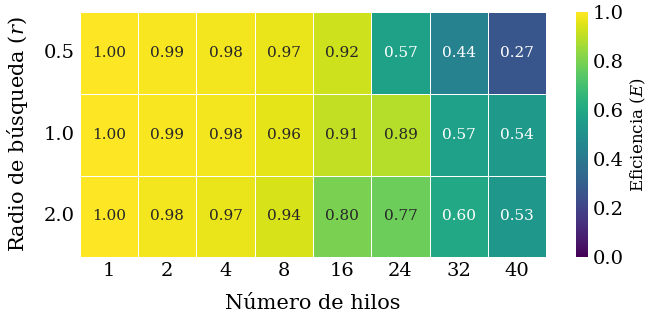
\includegraphics[width=\textwidth]{figuras/parallel/subset_paris_none.png}
        \caption{Algoritmo de búsqueda de Octree lineal base}
        \label{fig:subset_a}
    \end{subfigure}
    
    \vspace{0.5cm}
    
    \begin{subfigure}{0.8\textwidth}
        \centering
        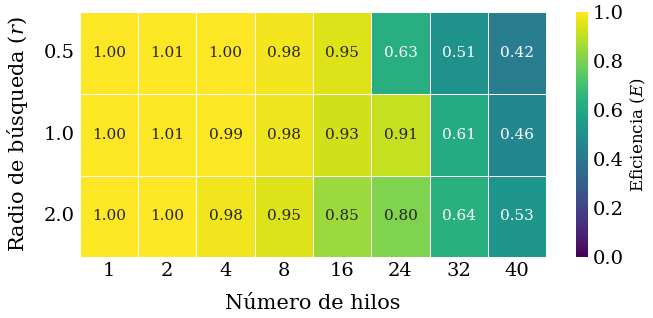
\includegraphics[width=\textwidth]{figuras/parallel/subset_paris_polar.png}
        \caption{Reordenamiento de las hojas del Octree en modo polar}
        \label{fig:subset_b}
    \end{subfigure}
    \vspace{0.5cm}
    \begin{subfigure}{0.8\textwidth}
        \centering
        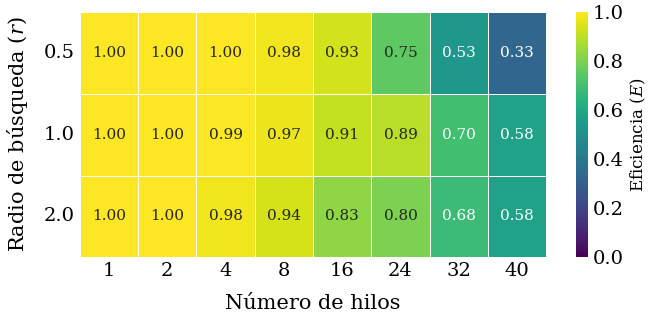
\includegraphics[width=\textwidth]{figuras/parallel/subset_paris_cartesian.png}
        \caption{Reordenamiento de las hojas del Octree en modo cartesiano}
        \label{fig:subset_c}
    \end{subfigure}
    
    % Caption global
    \caption{Mapas de calor de eficiencia de paralelización sobre centros aleatorios en la nube de puntos \textit{Paris\_Luxembourg \_6} }
    \label{fig:parallel_subset}
\end{figure}

Para terminar, se exponen en la Figura \ref{fig:parallel_full} los mapas de calor para el dataset \textit{Lille\_0}, sobre el que se realizaron búsquedas completas para los distintos reordenamientos. En estos \textit{heatmaps} se aprecia una paralelización muy potente, solamente bajando del 90\% de eficiencia en los casos más extremos, con más de 32 núcleos de procesamiento paralelos y radios cortos. De nuevo, se debe poner el foco en la zona superior derecha para observar los resultados más correlacionados con el funcionamiento general de la escalabilidad. Al igual que en las búsquedas aleatorias, las ejecuciones sin poda a nivel de hoja tienen peor eficiencia temporal en los casos más críticos de paralelización, sobre un 5\% más bajo que en los modos del reordenamiento polar y cartesiano, que tienen comportamientos casi idénticos entre sí.


\begin{figure}[htbp]
    \centering
    \begin{subfigure}{0.8\textwidth}
        \centering
        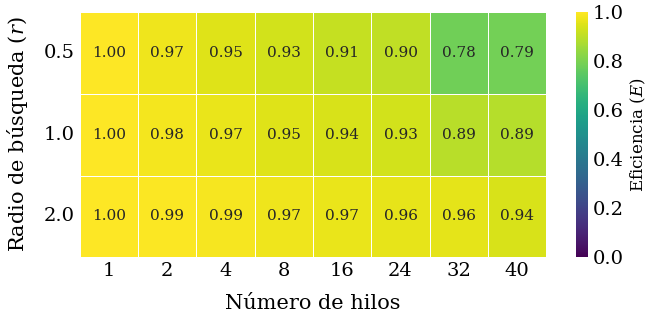
\includegraphics[width=\textwidth]{figuras/parallel/full_lille_none.png}
        \caption{Algoritmo de búsqueda de Octree lineal base}
        \label{fig:full_a}
    \end{subfigure}
    
    \vspace{0.5cm}
    
    \begin{subfigure}{0.8\textwidth}
        \centering
        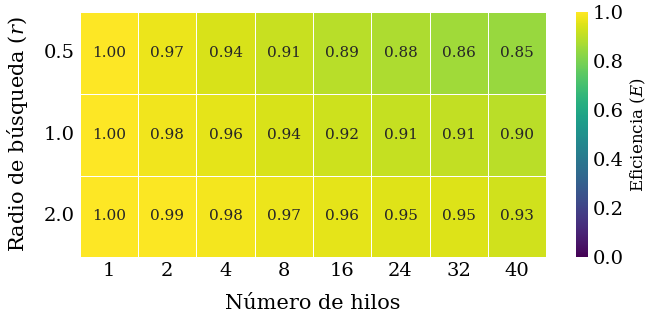
\includegraphics[width=\textwidth]{figuras/parallel/full_lille_polar.png}
        \caption{Reordenamiento de las hojas del Octree en modo polar}
        \label{fig:full_b}
    \end{subfigure}
    \vspace{0.5cm}
    \begin{subfigure}{0.8\textwidth}
        \centering
        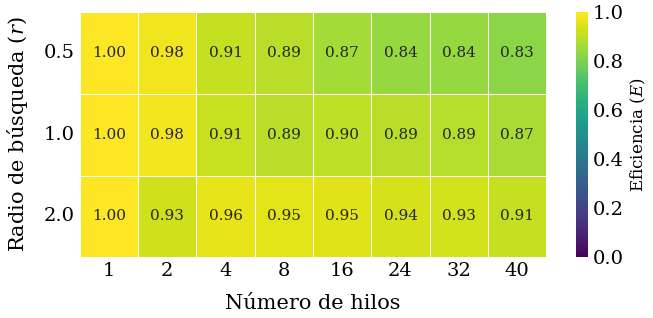
\includegraphics[width=\textwidth]{figuras/parallel/full_lille_cartesian.png}
        \caption{Reordenamiento de las hojas del Octree en modo cartesiano}
        \label{fig:full_c}
    \end{subfigure}
    
    % Caption global
    \caption{Mapas de calor de eficiencia de paralelización sobre coberturas completas en la nube de puntos \textit{Lille\_0} }
    \label{fig:parallel_full}
\end{figure}